\renewcommand{\thesection}{\Alph{section}}
\section{Implémentation de SAFE pour des modes de Lamb}

\subsection{Formalism}
\begin{enumerate}
    \item Variational form for elasticity equations
\begin{equation}
    - \rho \omega^2 \int_\Omega u \delta u \:d\Omega+ \int_\Omega \mbf \sigma (u) : \mbf \varepsilon (\delta u) \:d\Omega = \int_{\partial \Omega} \mbf \sigma (\delta u) \cdot \mbf n \:d\Gamma, \quad \forall \: \delta u
\end{equation}

\item Displacement fields $\mbf u (\mbf x) = \mbf u(x_2) e^{ik_1 x_1}e^{-i\omega t}$
    
\item Double dot product $\mbf \sigma (u) : \mbf \varepsilon (\delta u ^\star) = \sigma_{ij}(u) \varepsilon_{ij}(\delta u ^\star)$

\begin{equation}
    \begin{aligned}
        \sigma_{11}\varepsilon_{11} &= k_1^2 (\lambda + 2\mu) u_1 \delta u_1 + - ik_1 \lambda \nabla u_2 \delta u_1 \\
        \sigma_{12}\varepsilon_{12} &= \frac \mu 2 \left(-ik_1 \nabla u_1 \delta u_2 + \nabla u_1 \delta \nabla u_1 + k_1^2 u_2\delta u_2 + ik_1 u_2 \nabla \delta u_1)\right) \\
        \sigma_{22}\varepsilon_{22} &= ik_1 \lambda u_1 \nabla \delta u_2 + (\lambda + 2\mu) \nabla u_2 \nabla \delta u_2
    \end{aligned}
\end{equation}

\item Explicit form for the weak form of elasticity equations, 
\begin{equation}
    \begin{aligned}
        \int_\Omega - \rho \omega^2 &\left(u_1 \delta u_1 + u_2 \delta u_2 \right) + k_1^2 (\lambda + 2\mu) u_1 \delta u_1 - ik_1 \lambda \nabla u_2 \delta u_1 -ik_1 \mu \nabla u_1 \delta u_2 + \mu \nabla u_1 \delta \nabla u_1 \\ &+ \mu k_1^2 u_2\delta u_2 + ik_1 \mu u_2 \nabla \delta u_1) + ik_1 \lambda u_1 \nabla \delta u_2 + (\lambda + 2\mu) \nabla u_2 \nabla \delta u_2 \:d\Omega =0 \quad \forall \: \delta u
    \end{aligned}
\end{equation}
where $\nabla u_i$ denotes differentiation of the $i$-th component of the displacement along $x_2$. Note that the surface term initally expressed vanishes from the no-traction boundary condition.

\item Discretized fields 
\begin{equation}
    \mbf u (\mbf x) =\mbf N (\xi) \mbf U e^{ik_1 x_1}e^{-i\omega t},
\end{equation}
with $\mbf N$ containing the second-order Lagrange shape functions, and $\mbf U$ is the vector of displacement amplitudes.

\item Elementary matrices
\begin{equation}
    \begin{aligned}
        \mbf M^{(e)}   &= \frac{h}{2} \int_{-1}^1 \mbf N^\transp \mbf N \:d\xi, \quad
        \mbf K^{(e)}   = \frac 2 h \int_{-1}^1 \nabla \mbf N^{\transp} \nabla \mbf N d\xi,\\
        \mbf C_1^{(e)} &= \int_{-1}^1 \mbf N^{\transp}\nabla \mbf N \:d\xi, \quad
        \mbf C_2^{(e)} = \int_{-1}^1 \nabla^\transp \mbf N^{\transp} \mbf N \mbf U\:d\xi,\\
    \end{aligned}
\end{equation}

\item Discretization $\forall \delta \mbf U$, weak form for one element and rearranging the terms

\begin{equation}
    \begin{aligned}
        \int_{\Omega_e} & k_1^2 \Big(
         \mu \delta \mbf U_2^\transp \mbf M^{(e)} \mbf U_2
        + (\lambda + 2\mu) \delta \mbf U_1^\transp \mbf M^{(e)} \mbf U_1\Big)
        + ik_1 \Big( \mu \delta \mbf U_2^\transp \mbf C_1^{(e)} \mbf U
        - \mu \delta \mbf U_1^\transp \mbf C_2^{(e)} \mbf U_2 \\ &
        + \lambda \delta \mbf U_1^\transp \mbf C_1^{(e)} \mbf U_2
        - \lambda \delta \mbf U_2^\transp \mbf C_2^{(e)} \mbf U_1 \Big)
        + \mu \delta \mbf U_1^\transp \mbf K^{(e)} \mbf U_1
        + (\lambda + 2\mu) \delta \mbf U_2^\transp \mbf K^{(e)} \mbf U_2 
        \\ &-\rho \omega^2 \delta \mbf U_1^\transp \mbf M^{(e)} \mbf U_1 -\rho \omega^2 \delta \mbf U_2^\transp \mbf M^{(e)} \mbf U_2 \:d\Omega_e = 0
    \end{aligned}
\end{equation}


\item General form for the problem
\begin{equation}
    \left( k_1^2 \mbf A_2 + ik_1 \mbf A_1 + \mbf A_0 - \omega^2 \mbf M \right) \mbf U = 0.
\end{equation}
Rewrites as a generalized eigenvalue problem,
\begin{equation}
    \left[\begin{pmatrix}
         -\mbf A_1 & \mbf A_0 - \omega^2\mbf  M\\
         \mbf I & \mbf 0 
    \end{pmatrix} - k_1 \begin{pmatrix}
        \mbf A_2 & \mbf 0\\ \mbf 0 & \mbf I 
    \end{pmatrix}\right] \begin{pmatrix}
        k_1 \mbf U \\ \mbf U 
    \end{pmatrix} = 0
\end{equation}
\end{enumerate}


\begin{figure}[h!]
    \centering
    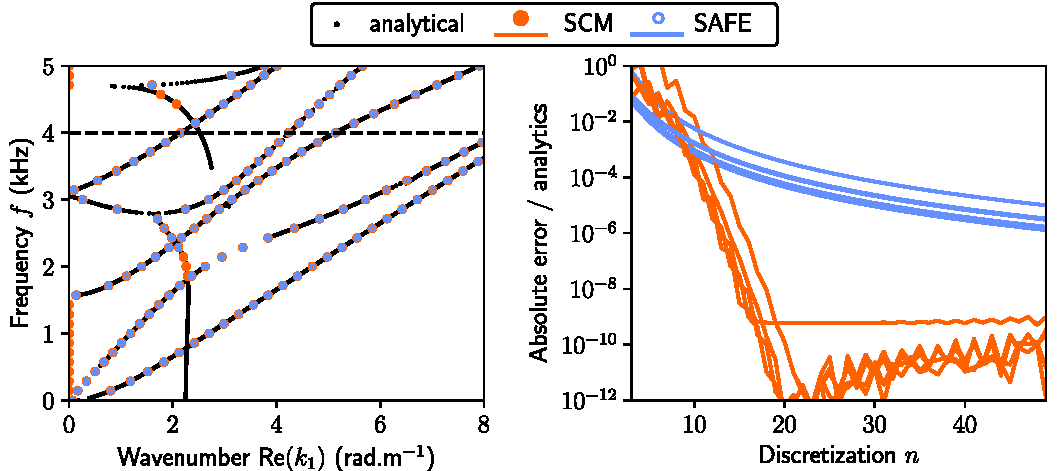
\includegraphics{./chapitres/annexes/figs/figure.pdf}
    \caption{a) Dispersion relation for the Lamb modes with the root-finding results, alongside the spectral collocation and semi-analytical finite elements solutions. b) Convergence curve of the 2 methods at a given frequency $f=4$ kHz. The multiple lines depicts the convergence of each wavenumber.}
    \label{fig:conv_scm_safe_lamb}
\end{figure}

\subsection{Results}
Analytical results are obtained by applying the root-finding approach using the Müller method presented in the paper. Solutions are sought from the classical Lamb modes equations, derived in many books such as Royer. Figure ~\ref{fig:conv_scm_safe_lamb}a) shows the results of the three methods for a given frequency range. They all match well. In order to compare the two numerical methods in play, a brief convergence study has been done using the analytical results from the root-finding method as a reference. 

The convergence curve of the results given in Fig.~\ref{fig:conv_scm_safe_lamb}b) is unsurprisingly in agreement with the literature. It is calculated at a frequency $f=4$ kHz: the solutions along the dashed line in Fig~\ref{fig:conv_scm_safe_lamb}a) are selected. The parameter $n$ used for the discretization is shared between the two methods and corresponds to the number of elements taken for the discretization in each method. SAFE matrices have a size $2(2n+ 1)$, with while SCM matrices have a size $2n$. The discretization is swept from $n=3$ to $n=50$.

The SCM convergence shows a steep slope and reaches a plateau around $n = 20$, while the SAFE curve follows the expected slope of a finite elements method that use second-order shape functions. When comparing at a given discretization order, the error from the SAFE is much lower that that of SAFE by several order of magnitudes. In order to see comparable convergence, it would require to use higher-order shape functions or use spectral elements instead.


\subsection{Point sur la biblio}
\begin{itemize}
    \item "Wave propagation along transversely periodic structures" cite \cite{predoi2007} 
    \item "Finite element model for waves guided along solid systems of arbitrary section coupled to infinite solid media" \cite{castaings2008} 
    \item "SAFE-PML approach for modal study of waveguides with arbitrary cross sections immersed in inviscid fluid" \cite{zuo2017} 
    \item "A coupled SAFE-2.5D BEM approach for the dispersion analysis of damped leaky guided waves in embedded waveguides of arbitrary cross-section" \cite{mazzotti2013} + "Dispersion analysis of leaky guided waves in fluid-loaded waveguides of generic shape" and \cite{mazzotti2014} "Dispersion analysis of leaky guided waves in fluid-loaded waveguides of generic shape"
    \item Livre J. Rose \cite{rose2014}
    \item Semi-Analytical Finite Element (SAFE) method for plotting Lamb waves dispersion curves of an aluminum plate and comparison with Disperse software \cite{yacoubi2022}
\end{itemize}